\chapter{Infinitesimalrechnung}

Die Infinitesimalrechnung beschäftigt sich mit der Analyse stetiger Funktionen. In diesem Kapitel werden wir zuerst die Ableitung und das Integral für ein- und mehrstellige Funktionen definieren. Anschließend betrachten wir Rechenregeln kennen lernen, mit den sich eine Funktion in der Praxis einfacher ableiten und integrieren lässt. Abschließend schauen wir uns noch an, wie mithilfe der Ableitung lokale Extremwerte bestimmt werden können.

\section{Begriff der Ableitung}

Motivation für den Ableitungsbegriff war es, beschreiben zu können, in welcher Art und wie schnell sich Funktionswerte an verschiedenen Stellen des Definitionsbereich ändern. Ein Auto, welches mit konstanter Geschwindigkeit fährt,  wird durch eine Gerade im Weg-Zeit-Diagramm beschrieben. Die Geschwindigkeit kann man jetzt auffassen als die Änderungsrate des Wegs bezüglich der Zeit, also wie viele Kilometer das Auto pro Stunde zurücklegt. Jetzt betrachten wir aber ein Auto, welches nicht mehr mit konstanter Geschwindigkeit fährt, sondern aus dem Stand von $0$ auf $100 \ukmh$ beschleunigt. Wie können wir nun die Geschwindigkeit definieren und messen? Aus der Erfahrung ist klar (wenn man auf das Tachometer schaut), dass die Geschwindigkeit zu jedem Zeitpunkt eine andere ist. Wir benötigen also eine Definition für die Geschwindigkeit zu \emph{einem Zeitpunkt}. Zu sagen, die Momentangeschwindigkeit sei die \emph{momentane Änderungsrate} des Wegs lässt zu wünschen übrig, denn wie kann sich der Weg zu einem Zeitpunkt ändern? Wir können uns diesem Problem nähern, indem wir uns zuerst klar machen, wie man die Geschwindigkeit in der Praxis messen würde. Wir würden messen, wie weit sich das Auto innerhalb eines kleinen Zeitintervalls, etwa $1$ Sekunde, fortbewegt hat und dann den zurückgelegten Weg durch die Zeit teilen. Wir erhielten damit einen Schätzwert für die Momentangeschwindigkeit innerhalb gewissen Fehlergrenzen. Um die Momentangeschwindigkeit besser zu messen, könnten wir das Zeitintervall verkleinern. Diese Idee, erst mit einem endlichen Zeitintervall zu beginnen und dieses dann zu verkleinern, ist die Grundidee für die mathematische Definition der Ableitung. Mittels des Grenzwertbegriffs können wir das Zeitintervall bis auf $0$ verkleinern und erhalten so die Geschwindigkeit als Ableitung der Weg-Zeit-Funktion.

\subsection{Ableitung einstelliger Funktionen}

\begin{definition}{Differenzierbarkeit und Ableitung}{DiffFun}
    Eine Funktion $f: \R \to \R$ heißt an der Stelle $x_0\in\mathcal{D}$ \textbf{ableitbar} (differenzierbar), wenn der Differenzenquotient konvergiert:
    $$
        \alpha = \lim\limits_{\varepsilon\to 0} \frac{f(x+\varepsilon) - f(x)}{\varepsilon}
    $$
    Dieser Grenzwert heißt dann \textbf{Ableitung der Funktion an der Stelle $x_0$} und man schreibt: $f'(x_0) = \alpha$.
    Falls eine Funktion auf ihrem gesamten Definitionsbereich differenzierbar ist, heißt sie \textbf{differenzierbare Funktion} und die durch
    $$
    f': x \mapsto \lim\limits_{\varepsilon\to 0} \frac{f(x+\varepsilon) - f(x)}{\varepsilon}
    $$
    definiert Funktion die \textbf{Ableitung} von $f$ nach $x$. Man schreibt auch dann gelegentlich auch $\dd{f}{x}$.
\end{definition}

Analog dazu definiert man auch die zweite Ableitung einer Funktion als die Ableitung der Ableitungsfunktion, die dritte Ableitung wieder als deren Ableitung und so weiter. Man schreibt $f''$ oder $\ddn{2}{f}{x}$ für die zweite Ableitung, $f'''$ oder $\ddn{3}{f}{x}$ für die dritte Ableitung. Für die $n$-te Ableitungen schreibt man statt den Strichen auch $f^{(n)}$ (man beachte die Klammern!).

\textbf{Anmerkung}: In der Physik schreibt man manchmal auch $\dot{f}$ für die \textbf{Ableitung einer Funktion nach der Zeit}.

\begin{figure}
    \centering
    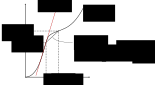
\includegraphics[width=0.8\textwidth]{./svg/derivative-function}
    \caption{Differenzenquotient einer Funktion}
    \label{fig:DiffFun}
\end{figure}

\begin{definition}{Lineare Näherung einer Funktion}{}
    Wenn eine Funktion $f$ an der Stelle $x_0$ differenzierbar ist, kann sie für kleine Abstände um diese Stelle herum durch eine Gerade $t$ genähert werden, welche man \textbf{Tangente} nennt und die gegeben ist durch:
    $$
        t: x \mapsto f(x_0) + f'(x_0) \cdot (x-x_0)
    $$
\end{definition}

Man kann sich auch vorstellen, man wählt sich eine Stelle $x_0$ und vergrößert den Graphen immer weiter um diese Stelle. Auch wenn die Funktion gesamt betrachtet gekrümmt sein mag, so wird sie, wenn sie denn differenzierbar ist, in der Vergrößerung aussehen wie eine Gerade. Diese Gerade nennt man dann Tangente.

\begin{example}{Bestimmung der Ableitung per Differenzenquotient}{DerivDiffQuot}
    Gesucht ist die Ableitung der Funktion $f(x) = x^2$ an einer Stelle $x_0$. Wir setzen in die Definition ein:
    \begin{alignat}{1}
        f'(x_0) &= \lim\limits_{\varepsilon\to 0} \frac{f(x_0+\varepsilon) - f(x_0)}{\varepsilon} \\
                &= \lim\limits_{\varepsilon\to 0} \frac{(x_0+\varepsilon)^2-x_0^2}{\varepsilon} \\
                &= \lim\limits_{\varepsilon\to 0} \frac{x_0^2+2x_0\varepsilon+\varepsilon^2-x_0^2}{\varepsilon} \\
                &= \lim\limits_{\varepsilon\to 0} 2x_0+\varepsilon \\
                &= 2x_0
    \end{alignat}
    Damit haben wir gezeigt, dass die quadratische Funktion überall differenzierbar ist und $f'(x) = \dd{}{x} x^2 = 2x$ gilt.
\end{example}

Eine wichtige Aussage über den Zusammenhang zwischen Stetigkeit und Differenzierbarkeit macht der folgende Satz:

\begin{statement}{Stetigkeit und Differenzierbarkeit}{ContDiffFun}
    Jede differenzierbare Funktion $f$ ist stetig. Die Stetigkeit ist also eine notwendige Bedingung für die Differenzierbarkeit, jedoch keine hinreichende Bedingung.
\end{statement}

\begin{example}{Stetige nicht differenzierbare Funktionen}{ContNonDiffFun}
    Die Betragsfunktion $f(x) = |x|$ ist für alle reellen Zahlen definiert und dort überall stetig. Speziell ist sie auch an der Stelle $x_0=0$ stetig. Allerdings ist sie dort nicht differenzierbar, denn
    der Grenzwert
    $$
        \lim\limits_{\varepsilon\to 0} \frac{f(0+\varepsilon) - f(0)}{\varepsilon} = \lim\limits_{\varepsilon\to 0} \frac{|\varepsilon|}{\varepsilon} = \lim\limits_{\varepsilon\to 0} \text{sgn}(\varepsilon)
    $$
    existiert nicht (siehe Beispiel \ref{ex:ExamContUnivarFun}). Graphisch betrachtet hat die Betragsfunktion bei $0$ einen Knick, der bestehen bleibt, egal, wie weit man den Knick vergrößert (sich also nicht als Gerade annähern lässt).
\end{example}

Es sei angemerkt, dass es auch Funktionen gibt, die überall stetig aber nirgends differenzierbar sind, ein Beispiel dazu findet sich im Anhang \ref{fig:BlancmangeFunction}.

Für viele Zusammenhänge ist es erforderlich, dass auch Ableitung selbst wieder eine stetige Funktion ist. Man definiert daher:

\begin{definition}{Stetige Differenzierbarkeit}{ContDiff}
    Eine Funktion $f$ heißt stetig differenzierbar, wenn sie differenzierbar ist und ihre Ableitung eine stetige Funktion ist.
\end{definition}

\begin{example}{Physikalische Anwendung der Ableitung}{}
    Eine Kreisbewegung in der $x$-$y$-Ebene mit konstanter Winkelgeschwindigkeit $\omega$ wird beschrieben durch $x(t) = r \cos(\omega t)$ und $y(t) = r \sin(\omega t)$, wobei $t$ die Zeit und $r$ den Radius des Kreises meint. Die erste Ableitung nach der Zeit lautet $v_x(t) = \dot{x}(t) = -r \omega \sin(\omega t)$, $v_y(t) = \dot{y}(t) = r \omega \cos(\omega t)$. Dabei handelt es sich um die x- und y-Komponenten der Geschwindigkeit $\vec v$, deren Betrag durch $|\vec v| = \sqrt{v_x^2+v_y^2} = r \omega$ gegeben ist. Damit haben wir die Formel für die Geschwindigkeit einer kreisförmigen Bewegung erhalten: $v = \omega r = 2\pi f r = \frac{2\pi r}{T}$ ($f\dots$Frequenz, $T\dots$ Periodendauer). Weiter können wir die zweite Ableitung bilden: $a_x(t) = \ddot{x}(t) = -r\omega^2 \sin(\omega t)$, $a_y(t) = \ddot{y}(t) = -r \omega^2 \sin(\omega t)$. Wir erhalten die x- und y-Komponenten der Beschleunigung $\vec a$, deren Betrag $|\vec a| = r \omega^2$ lautet. Das ist die Formel für die Beschleunigung bei einer Kreisbewegung: $a = \omega^2 r = \frac{v^2}{r}$. Die Zentripetalkraft (beziehungsweise Zentrifugalkraft in einem mitbewegten Inertialsystem) beträgt dann $F_Z = m \cdot a = m \frac{v^2}{r}$.
\end{example}

\subsection{Ableitung mehrstelliger Funktion}

Bisher haben wir die Ableitung nur für einstellige Funktionen betrachtet. Für mehrstellige Funktionen gibt es ein analoges Konzept, welches man die partielle Ableitung nennt. Der Funktionswert einer mehrstelligen Funktion wie etwa $f(x,y) = x^2+y^2$ hängt von mehreren Argumenten ab. Wir können aber alle Argumente bis auf eines festhalten (auf einen konstanten Wert setzen) und erhalten so wieder eine einstellige Funktion. Also beispielsweise $f(x,2) = x^2+4$. Diese einstellige Funktion entspricht einem Querschnitt durch den Graphen der zweistelligen Funktion, in diesem Fall dem Querschnitt durch die Ebene parallel zur $x$-$z$-Ebene. Ebenso hätten wir auch $x$ festhalten können und würden etwa $f(3, y) = y^2+9$ erhalten. Diese einstelligen Funktionen kann man nun ableiten und erhält die sogenannten partiellen Ableitungen, welche die Änderungsrate einer mehrstelligen Funktion in einer bestimmten Richtung beschreiben.

\begin{definition}{Partielle Ableitung}{PartDerivFun}
    Sei $f: \R^n\to\R$ eine mehrstellige Funktion. Die \textbf{partielle Ableitung} von $f$ nach $x_i$ ($1<i<n$) wird definiert als die Ableitung der einstelligen Funktion nach $x_i$, die entsteht, wenn man alle Argumente außer $x_i$ konstant hält. Man schreibt:
    \begin{alignat*}{1}
        \pdd{f}{x_i} \text { oder } f_{x_i} & \text{ für die erste Ableitung nach } x_i \\
        \pddn{2}{f}{x_i x_j} \text {oder } f_{x_i,x_j} & \text{ für die zweite Ableitung nach } x_i \text{ und } x_j
    \end{alignat*}
\end{definition}

Hierbei ist unbedingt auf die Reihenfolge der Ableitungen aufzupassen. $f_{xy}$ bezeichnet die Ableitung einer zweistelligen Funktion zuerst nach $x$ und dann nach $y$, $f_{yx}$ die Ableitung erst nach $y$ und anschließend nach $x$.

\begin{example}{Partielle Ableitungen}{PartDiff}
    \begin{itemize}
        \item Die partielle Ableitungen von $f(x,y) = x^2+y^2$ erhält man, indem man $x$ beziehungsweise $y$ als Konstante betrachtet und die Rechenregeln für das Differenzieren einstelliger Funktionen anwendet: $f_x = 2x$, $f_y = 2y$, $f_{xx} = 2$, $_{yy} = 2$.
        \item Die partielle Ableitung $f_z$ von $f(x,y) = \sin(x+\ln(y))$ lautet $f_z = 0$, da $z$ überhaupt nicht in $f$ vorkommt, die Funktionswerte sich somit bei Änderungen von $z$ nicht ändern.
    \end{itemize}
\end{example}

Im Beispiel \ref{ex:PartDiff} sehen wir, dass die beiden partiellen $f_{xy}$ und $f_{yx}$ übereinzustimmen scheinen, die Reihenfolge der Ableitungen also keine Rolle spielt. Es stellt sich daher die Frage, ob dies eine Ausnahme ist oder verallgemeinert werden kann. Der folgende Satz gibt darüber Auskunft:

\begin{statement}{Satz von Schwarz}{SchwarzTheo}
    Sei $f: \R^n \to \R$ ein mehrstelligen Funktion deren zweite partielle Ableitungen $f_{x_i x_j}$ und $f_{x_j x_i}$ stetig sind. Dann sind diese beiden Ableitungen gleich:
    $$
      f_{x_i x_j}, f_{x_j x_i} \text{ stetig}: \implies f_{x_i x_j} = f_{x_j x_i}
    $$
\end{statement}

$\pdd{f}{x}$ bezeichnet die partielle Ableitung eine bestimmten Funktion nach $x$. Um auszudrücken, dass man sich auf die Rechenoperation "\emph{Eine Funktion nach x ableiten}" bezieht, schreibt man $\pdd{}{x}$. Dieser Ausdruck ist ein sogenannten ¸\emph{Operator}, welcher auf beliebige Funktionen angewandt werden kann und eine neue Funktion zurückliefert, nämlich deren Ableitung nach $x$. Analog dazu ist $\dd{}{x}$ der \emph{Differentialoperator}, der einer einstelligen Funktion ihre Ableitung zuordnet.

Für mehrstellige Funktionen definiert man noch den sogenannten \mention{Nabla}-Operator, welcher sich zusammensetzt aus den einzelnen partiellen Ableitungen:

\begin{definition}{Nabla-Operator}{NablaOp}
    Für eine $n$-stellige Funktion bezeichnet $\vec \nabla = \rvec{\pdd{f}{x_1}}{\vdots}{\pdd{f}{x_n}}$ den Nabla-Operator. Dieser verhält sich wie ein Vektor und ordnet bei Anwendung auf eine Funktion ihr einen Vektor aus den partiellen Ableitungen zu.
\end{definition}

Dieser Operator ist nützlich, da er viele Formeln der Infinitesimalrechnung mehrstelliger Funktionen vereinfacht. Im letzten Kapitel haben wir bereits gesehen, dass man das Gradientenfeld einer mehrstelligen Funktion damit bündig schreiben kann als $\vec\nabla f$. Besonders bei Funktionen $\R^n \to \R^n$ wird der Nabla-Operator häufig verwendet. Da wir uns in dieser Vorlesung auf Funktionen $\R^n\to\R$ beschränken, werden wir den Nabla-Operator im Rahmen dieser Vorlesung kaum brauchen.

Schließlich können wir analog zur Tangenten für einstellige Funktionen noch eine sogenannten \emph{Tangentialebene} für zweistellige Funktionen definieren, also eine Ebene, die sich an die Funktion in einem Punkt anschmiegt. Diese Tangentialebene erhalten wir, wenn wir eine Ebene aufspannen, welche in $x$- und $y$-Richtung jeweils den Anstieg der Funktion in dieser Richtung hat. Dieser Anstieg ist durch die partiellen Ableitungen gegeben. Dieses Vorgehen lässt sich allgemein auf $n$-stellige Funktionen erweitern.

\begin{definition}{Lineare Näherung einer mehrstelligen Funktion}{LinApproxMultivarFun}
    Sei $f: \R^n\to\R$ ein $n$-stellige, partiell differenzierbare Funktion. Dann heißt $t$ die \textbf{lineare Näherung} der Funktion in einer kleinen Umgebung um einen Punkt $\vec{r_0}\in\R^n$ und ist gegeben durch:
    $$
        t(\vec r) = f(\vec{r_0}) +  \vec{\nabla}f(\vec{r_0}) \cdot (\vec{r} - \vec{r_0})
    $$
    Speziell für zweistellige Funktion $f(x,y)$ heißt $t$ die \textbf{Tangentialebene} und berechnet sich als:
    $$
        t(x,y) = t(x_0,y_0) + f_x(x_0,y_0) \cdot (x-x_0) + f_y(x_0,y_0) \cdot (y-y_0)
    $$
\end{definition}

Man beachte besonders, dass diese Formel für die lineare Näherung einer mehrstelligen Funktion identisch mit der Formel für die Tangentengleichung einer einstelligen Funktion ist, wenn man $n=1$ setzt.

\begin{example}{Bestimmung der linearen Näherung einer Funktion}{CompTangPlane}
    Gegeben sei die Funktion $f(x,y,z) =x^2+y^2+z$. Wir suchen die Gleichung der linearen Näherung an der Stelle $\vec{r_0} = (2,4,1)$. Um die Formel \ref{def:LinApproxMultivarFun} anwenden zu können, berechnen wir zuerst $\vec\nabla f$:
    $$
        \vec\nabla (x^2+y^2+z^2) = \rvec{\pdd{}{x} (x^2+y^2+z)}{\pdd{}{y} (x^2+y^2+z)}{\pdd{}{z} (x^2+y^2+z)} = \rvec{2x}{2y}{1}
    $$
    Dies setzen wir in die Formel ein und erhalten:
    \begin{alignat*}{1}
        t(x,y,z) &= t(x_0,y_0,z_0) + \rvec{2\cdot x_0}{2\cdot y_0}{z_0} \cdot \rvec{x-x_0}{y-y_0}{z-z_0} \\
                 &= t(2,4,1) + \rvec{2\cdot 2}{2\cdot 4}{1} \cdot \rvec{x-2}{y-4}{z-1} \\
                 &= 21 + 4 (x-2) + 8 (y-4) + (z-1)
    \end{alignat*}
\end{example}

Mittels der partiellen Ableitung lassen sich auch einige geometrische Sachverhalte ausdrücken. Als Beispiel wollen wir einen Berggipfel betrachten. Wir nehmen an, dass wir dessen Form in ersten Näherung durch $f(x,y)=1-x^2-y^2$ beschreiben können. Wenn wir nun eine Kugel nehmen, an eine Stelle platzieren und loslassen, wird die Kugel nach unten rollen. Doch in welche Richtung genau wird sie rollen? Aus der Erfahrung wissen wir, dass die Kugel nicht spiralförmig nach unten rollt, sondern auf dem direkten Weg nach unten. Diese Richtung entspricht der Richtung des stärksten Abfalls des Berggipfels. Mathematisch können wir diese Richtung durch den sogenannten Gradient berechnen, welcher aus den partiellen Ableitungen besteht:

\begin{definition}{Gradient}{Gradient}
	Der \textbf{Gradient} einer $n$-stelligen Funktion $f: \R^n \to  \R$ an einer Stelle $\vec{r}$ ist ein $n$-stelliger Vektor, welcher in die Richtung des stärksten Anstiegs an dieser Stelle zeigt und dessen Betrag ein Maß für die Größe des Anstiegs ist:
	$$
		\grad(f)(\vec{r}) = \vec\nabla f(\vec{r}) = \rvec{\pdd{f}{x_1}(\vec{r})}{\vdots}{\pdd{f}{x_n}(\vec{r})}
	$$
\end{definition}

Dabei müssen wir beachten, dass der Gradient in die Richtung des stärksten Anstiegs (nicht Abfalls) zeigt. Für unser Beispiel mit dem Berggipfel wird die Kugel also in die entgegengesetzt Richtung des Gradienten rollen, siehe Beispiel \ref{ex:GradField}. Der Gradient entspricht auch der mathematischen Definition des Richtungsfelds, welches wir im letzten Kapitel in Definition \ref{def:GradField} kennengelernt haben.

\begin{example}{Richtungsfeld einer Funktion}{GradField}
	Gesucht ist das Richtungsfeld der zweistelligen Funktion $f(x,y) = 1-x^2-y^2$. Gemäß Definition müssen wir zuerst die beiden partiellen Ableitungen nach $x$ und $y$ berechnen:
	\begin{alignat*}{1}
	\pdd{}{x} x^2+y^2 &= -2x \\
	\pdd{}{y} x^2+y^2 &= -2y
	\end{alignat*}
	Damit lässt sich das Richtungsfeld $G: \R^2 \to \R^2$ nun angeben als:
	$$
	G(x,y) = \grad f = \tvec{-2x}{-2y}
	$$
	Die Richtung des stärksten Anstiegs verläuft wie in Abbildung \ref{fig:ExGradField} zu sehen also immer radial weg vom Koordinatenursprung. Aus der Anschauung ist dies unmittelbar klar, bei dem Graphen von $f$ handelt es sich um einen nach unten geöffnete Kesselform beziehungsweise einen "Berggipfel". An der Stelle $(1,1)$ etwa ergibt sich $G(1,1) = \tvec{-2}{-2}$. Das ist aber bergauf in Richtung des Berggipfels. Die Richtung des stärksten Abfalls ist genau entgegengesetzt: $-G(1,1) = \tvec{2}{2}$. 	
\end{example}

Abschließend sei erwähnt, dass es auch weitere Operationen gibt, wie etwa der sogenannten Divergenz $\text{div} \vec{F} = \vec{\nabla} \cdot \vec{F}$ oder der Rotation $\text{rot} \vec{F} = \vec{\nabla} \times \vec{F}$. Diese operieren auf vektorwertigen Funktionen (Feldern), also Funktionen, bei denen die Funktionswerte nicht reelle Zahlen sind, sondern aus Vektoren bestehen. In der Physik sind etwa das elektrische und magnetische Feld Funktionen $f: \R^3 \to \R^3$, die jedem Punkt im Raum einen Feldvektor zuordnen. Diese Art von Funktionen werden wir aber im Rahmen dieser Vorlesung nicht weiter betrachten.

\section{Begriff des Integrals}

\subsection{Einstellige Funktionen}

Die Ableitung können wir uns graphisch vorstellen als das Anlegen einer Tangente an eine Funktion. Ebenso könnten wir uns dem Integralbegriff über eine geometrische Fragestellung nähern. Wir betrachten zunächst einmal die Funktion $f(x) = \sin(x)$. Diese hat jeweils bei $0$ und bei $\pi$ eine Nullstelle. Wir stellen uns nun die Frage, wie groß der Flächeninhalt ist, den die Sinuskurve zwischen $0$ und $\pi$ mit der x-Achse einnimmt.

Um uns dieser Frage zu nähern, gehen wir auf ähnliche Weise zur Ableitung vor. Dort hatten wir zuerst Sekanten betrachtet und dann eine Grenzwertbildung vorgenommen, um die exakte Tangente zu erhalten. Genauso können wir für den Flächeninhalt mit einer Näherung anfangen, indem wir den Flächeninhalt unter der Sinuskurve durch kleine Rechtecke annähern, wie dies in Abbildung \ref{fig:ApproxAreaUnivarFun} dargestellt ist.

\begin{figure}
    \centering
    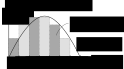
\includegraphics[width=0.6\textwidth]{./svg/integral-univariate-function}
    \caption{Annäherung des Flächeninhalts über Rechtecke}
    \label{fig:ApproxAreaUnivarFun}
\end{figure}

Wir zerlegen das Intervall $[a, b] = [0,\pi]$, für dem wir in den Flächeninhalt berechnen wollen, in die $n$ Teilintervalle $[x_i, x_{i+1}]$ ($0\le i \le n)$ mit der Länge $\Delta x_n = \frac{b-a}{n}$ . Dabei sind $x_i$ die Stützpunkte, welche sich ergeben zu $x_i = a + i\cdot\frac{b-a}{n} \cdot b$. Der Flächeninhalt $A_i$ ($1\le i \le n$) des $i$-ten Rechtecks berechnet sich als Breite mal Höhe. Die Breite ist gleich $\Delta x$, die Höhe entspricht dem Funktionswert $f(x_i)$ am $i$-ten Stützpunkt: $A_i = \Delta x \cdot f(x_i)$. Den gesamten Flächeninhalt $A$ erhalten wir, indem wir nun den Flächeninhalt aller Rechtecke aufaddieren:

\begin{alignat*}{1}
  A_n = \sum_{i=0}^{n-1} A_i &= \sum_{i=1}^{n} \frac{b-a}{n} f(a + i\cdot\frac{b-a}{n}) \\
                             &= \sum_{i=1}^{n} \Delta x_n f(a + i\cdot\Delta x) \\
\end{alignat*}

In Tabelle \ref{lst:ApproxIntegral} sind die Näherungswerte für einige $n$ angegeben.

\begin{listing}
    \begin{center}
        \begin{tabular}{ r | l}
            \textbf{Teilintervalle $n$} & \textbf{Näherungswert $A_n$} \\
            \hline
            1 & 0.00000 \\
            2 & 1.57079\dots \\
            3 & 1.81379\dots \\
            4 & 1.89611\dots \\
            5 & 1.93376\dots \\
            6 & 1.95409\dots \\
            7 & 1.96631\dots \\
            8 & 1.97423\dots \\
            9 & 1.97965\dots
        \end{tabular}
    \end{center}
    \caption[Näherungsweise Berechnung eines bestimmen Integrals]{Näherungswerte für den Flächeninhalt eingeschlossen durch den Graphen von $\sin(x)$ mit der x-Achse zwischen $0$ und $pi$.}
    \label{lst:ApproxIntegral}
\end{listing}

Wir sehen, je größer wir die Anzahl der Teilintervalle wählen, desto besser wird die Näherung (der genaue Wert lautet $2$). Mathematisch können wir dies fassen, in dem wir den Grenzwert für $n \to \infty$ bilden. Dies bringt uns zur Definition des bestimmten Integrals:

\begin{definition}{Bestimmtes Integral}{DefInteg}
    Das \textbf{bestimmte Integral} einer stetigen Funktion $f: \R \to \R$ im Intervall $[a,b] \subset \R$ ist der Grenzwert der Flächeninhaltssummen $A_n$, falls dieser existiert:
    $$
        \int\limits_{a}^b f(x) \diff{x} = \lim\limits_{n\to\infty} \sum_{i=1}^{n} \Delta x_n f(a + i\cdot\Delta x)
    $$
    Graphisch entspricht das bestimmte Integral dem \textbf{gerichteten Flächeninhalt} zwischen dem Graphen von $f$ unter der Abszisse (x-Achse). Der gerichtete Flächeninhalt ist positiv, wenn die Fläche oberhalb der Abszisse liegt, und negativ, wenn sie unterhalb der Abszisse liegt.
\end{definition}

\begin{example}{Berechnung des bestimmten Integrals}{CompDefInteg}
    \begin{itemize}
        \item Gesucht ist der Flächeninhalt zwischen $f(x) = x^2$ unter der x-Achse im Intervall $[0,1]$. Die Intervallänge lautet $\Delta x_n = \frac{b-a}{n} = \frac{1}{n}$. Die Funktionswerte an der Stützstelle $x_i = a + i \Delta x = \frac{i}{n}$ lauten $f(x_i) = \frac{i^2}{n^2}$. Eingesetzt in die Definition erhalten wir damit:
        \begin{alignat*}{1}
            A &= \lim\limits_{n\to\infty} \sum_{i=1}^{n} \Delta x_n f(a + i\cdot\Delta x) \\
              &= \lim\limits_{n\to\infty} \sum_{i=1}^{n} \frac{1}{n} \frac{i^2}{n^2} \\
              &= \lim\limits_{n\to\infty} \frac{1}{n^3} \sum_{i=1}^{n} i^2 \\
              &= \lim\limits_{n\to\infty} \frac{n^3/3+n^2/2+n/6}{n^3} \\
              &= \lim\limits_{n\to\infty} \frac{1}{3} + \frac{1}/{2n} + \frac{1}/{6n^2} \\
              &= \frac{1}{3}
        \end{alignat*}
        Wir haben dabei von der Formel zur Addition der Quadratzahlen Gebrauch gemacht: $1^2 + 2^2 + 3^2 + \dots + n^2 = \frac{n (n+1) (2n+1)}{6}$.
        \item Das bestimmte Integral über $\sin(x)$ zwischen $0$ und $2\pi$ lautet $0$, da der Flächeninhalt aus zwei betragsmäßig gleichen Teilen besteht, wobei der eine überhalb der x-Achse liegt und der andere Teil unterhalb der x-Achse. Der gerichtete Flächeninhalt des linken Teils ist somit positiv, der des rechten Teils, und in der Summe ergibt sich $0$.
    \end{itemize}
\end{example}

Nun ist es in der Praxis meist recht mühselig, jedesmal den Grenzwert ermitteln zu müssen. Glücklicherweise gibt es eine weitere Weise, das unbestimmte Integral zu berechnen. Dazu benötigen wir zuerst einmal die folgende Definition, welche man verstehen kann als Umkehroperation zum Differenzieren:

\begin{definition}{Stammfunktion und unbestimmtes Integral}{AntiDerivative}
    Eine Funktion $F$ heißt \textbf{Stammfunktion zu $f$}, wenn $f$ die Ableitung von $F$ ist: $\dd{F}{x} = f$. Die Menge aller Stammfunktionen nennt man das \textbf{bestimmte Integral} von $f$ und schreibt:
    $$
        \int f(x) \diff{x} = F(x) + C
    $$
    Dabei ist $C \in \R$ eine beliebige Konstante.
\end{definition}

Man beachte hierbei, dass es im Allgemeinen unbegrenzt viele Stammfunktionen gibt. Wenn $F$ eine Stammfunktion ist, kann man immer eine neue Funktion durch Addition mit einer konstanten Zahl bilden. Diese ist ebenfalls eine Stammfunktion, da das Addieren einer Konstant einem Verschieben der Funktion entlang der y-Achse entspricht und die Änderungsrate der Funktion nicht beeinflusst.

Der folgende Satz macht nun eine erstaunliche Aussage über den Zusammenhang zwischen dem bestimmten und dem unbestimmten Integral:

\begin{definition}{Hauptsatz der Differential- und Integralrechnung}{FundTheoCalc}
    Sei $F$ eine Stammfunktion von $f$, dann ist das bestimmte Integral im Intervall $[a,b]$  gleich der Differenz der Funktionswerte der Stammfunktion an den Intervallgrenzen:
    $$
        \int\limits_a^b = \left[F(x)\right]_a^b = F(b) - F(a)
    $$
\end{definition}

\begin{example}{Berechnung des bestimmten Integrals per Stammfunktion}{CompDefIntAntiDer}
    \begin{itemize}
        \item $F(x) = \frac{1}{3}x^3$ ist eine Stammfunktion von $f(x)=x^2$, wie man durch Ableiten von $F$ nachprüft. Der bestimmte Integral $\int\limits_0^1 x^2 \diff{x}$ ergibt sich somit zu $F(1)-F(0) = \frac{1}{3}$.
        \item Für $f(x) = \sin(x)$ ist $F(x) = -\cos(x)$ eine Stammfunktion. Somit ergibt sich für das bestimmte Integral $\int\limits_0^\pi \sin(x) = \left[-\cos(x)\right]_0^\pi = -\cos(\pi) - (-\cos(0)) = 2$.
    \end{itemize}
\end{example}

Eine wichtige Eigenschaft des bestimmten Integrals ist die Additivität der Grenzen. Wenn wir beispielsweise den (gerichteten) Flächeninhalt in den Intervallen $[0,1]$ und $[1,2]$ kennen, können wir daraus auch den (gerichteten) Flächeninhalt im Intervall $[0,2]$ ableiten, in dem wir die beiden einzelnen Flächeninhalt aufaddieren.

\begin{statement}{Additivität der Grenzen des bestimmten Integrals}{AddBoundDefInt}
    Das unbestimmte Integral einer Funktion $f$ über von $a$ bis $c$ lässt sich aufteilen in zwei unbestimmte Integrale mit einem Zwischenwert $b$:
    $$
    \int\limits_a^b f(x) \diff{x} + \int\limits_b^c f(x) \diff{x} = \int\limits_a^c f(x) \diff{x}
    $$
    Dies ist sogar dann gültig, wenn $b$ nicht zwischen $a$ und $c$ liegt.
\end{statement}

Der Beweis dazu folgt sofort aus dem Hauptsatz:

$$
    \int\limits_a^b f(x) \diff{x} + \int\limits_b^c f(x) \diff{x} = F(b) - F(a) + F(c) - F(b) = F(c) - F(a) = \int\limits_a^c f(x) \diff{x}
$$

\subsection{Mehrstellige Funktionen}


Nachdem wir uns nun angeschaut haben, wie man bestimmte Integrale eindimensionaler Funktionen berechnet, wollen wir den Begriff des bestimmten Integrals noch auf zweistellige Funktionen erweitern. Dies ist ein komplexes Themengebiet und daher hier nur auszugsweise dargestellt.

Um zu verstehen, was es bedeutet, eine zweistellige Funktion zu integrieren, erinnern wir uns nochmal, wie wir bei einstelligen Funktionen vorgegangen sind. Einstellige Funktionen haben eine Teilmenge der reellen Zahlen $\R^1$ als Definitionsbereich. Für die Definition des bestimmten Integrals haben wir diese eindimensionale Teilmenge (eine Gerade) in kleine Geradenstücke zerlegt. Für jedes Geradenstück haben wir dann dessen Länge $\Delta x$ multipliziert mit dem Funktionswert an dieser Stelle. Schließlich haben wir diese Werte alle aufaddiert.

Ersetzen wir nun "Gerade" durch "Fläche", "Geradenstück" durch "Flächenstück" und "Länge" durch "Flächeninhalt", erhalten wir die graphische Bedeutung des bestimmten Integrals einer zweistelligen Funktion $f(x,y)$ -- das Volumen, das der Graph der Funktion mit der x-y-Ebene einnimmt. Statt über ein eindimensionales Intervall zu integrieren, führen wir die Integration nun über eine Flächenstück der x-y-Ebene aus. Diese zerlegen wir in viele kleine Flächenstücke. Für jedes Flächenstück multiplizieren wir dessen Flächeninhalt mit dem Wert der Funktion an dieser Stelle und erhalten dadurch das Volumen des kleiner Quaders über diesem Rechteck. Abschließend addieren diese Werte auf.

Diese Vorgehensweise wollen wir uns noch anhand einer rechteckigen und eines kreisförmigen Fläche anschauen.

\subsection{Gebietsintegral in kartesischen Koordinaten}


Der Fall für eine rechteckige Fläche ist dargestellt in Abbildung \ref{fig:AreaIntegCartesian}.

\begin{figure}
    \centering
    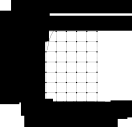
\includegraphics[width=0.48\textwidth]{./svg/integral-2d-cartesian}
    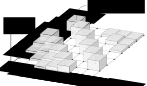
\includegraphics[width=0.48\textwidth]{./svg/integral-2d-cartesian-perspective}
    \caption[Gebietsintegral in kartesischen Koordinaten]{Graphische Interpretation eines Gebietsintegrals in kartesischen Koordinaten. Der Funktionswert an jedem kleinen schwarzen Punkt wird mit dem Flächeninhalt des Rechtecks multipliziert.}
    \label{fig:AreaIntegCartesian}
\end{figure}

Wir zerlegen nun analog zu einstelligen Funktionen das Rechteck $[a,b] \times [c,d]$, über das wir integrieren wollen, in $n\cdot m $ kleine Rechtecke $[x_i,x_{i+1}] \times [y_j,y_{j+1}]$. Jedes kleine Rechteck hat die Seitenlängen $\Delta x = \frac{b-a}{n}$ und $\Delta y = \frac{d-c}{m}$. Der Flächeninhalt des kleinen Rechtecks beträgt damit $A_{nm} = \Delta x \Delta y = \frac{(b-a)(c-d)}{nm}$. Die Stützpunkte lauten nun $x_i = a + i \Delta x$ und $y_j = c + j \Delta y$.  Nun multiplizieren wir den Flächeninhalt des Rechtecks mit dem Funktionswert und bilden die Summe. Wir erhalten:

\begin{center}
    \begin{alignat*}{1}
          & \lim\limits_{(n,m) \to (\infty, \infty)} \sum\limits_{j=1}^m \sum\limits_{i=1}^n f(x_i,y_j) \Delta x_n \Delta y_m  \\
        = & \int\limits_c^d \int\limits_a^b f(x,y) \diff{x} \diff{y}
    \end{alignat*}
\end{center}

Das letzte Gleichheitszeichen folgt aus der Definition des bestimmten Integrals für einstellige Funktionen. Wir sehen also, dass man ein mehrstelliges Integral durch Hintereinanderausführung normaler Integrale berechnen können. Statt über ein rechteckiges Gebiet zu integrieren, können wir auch über ein andersförmiges Gebiet integrieren, indem wir die Grenzen für die Integration über $x$ nicht auf einen festen Wert setzen, sondern von $y$ abhängen lassen (oder umgedreht). Wir erhalten damit das Gebietsintegral in kartesischen Koordinaten:

\begin{definition}{Gebietsintegral in kartesischen Koordinaten}{AreaIntCartCoord}
    Seien $u,v$ zwei einstellige Funktionen und $y_1,y_2\in\R$ zwei feste Zahlen. Dann wird durch $A = \left\lbrace (x,y) \in \R^2 | y \in [y_1,y_2] \land x \in [l(y), u(y)] \right\rbrace$ eine zweidimensionale Fläche beschrieben. Das Gebietsintegral einer Funktion $f$ über diese Fläche $A$ berechnet sich dann als:
    $$
        \int\limits_{A} f(x,y) \diff{A} = \int\limits_{y_1}^{y_2} \int\limits_{l(y)}^{u(y)} f(x,y) \diff{x} \diff{y}
    $$
\end{definition}

\begin{example}{Gebietsintegral in kartesischen Koordinaten}{AreaIntCarCoordTetra}
    Wir betrachten eine dreiseitige schiefe Pyramide, deren Spitze im Koordinatenursprung liegt und in Abbildung \ref{fig:AreaIntegTetraeder} dargestellt ist. Wir wollen das Volumen von diesem Körper berechnen. Der obere Punkte des Körpers in Abhängigkeit von $x$ und $y$ lautet $f(x,y) = 1-x-y$. $y$ bewegt sich dabei in den Grenzen $[0,1]$. Das Intervall für $x$ ist abhängig vom Wert von $y$. Die Untergrenze $l(y) = 0$ ist fest, die Obergrenze ist $u(y) = 1 - y$. Für das Volumen folgt nun unter über das Gebietsintegral:
    \begin{alignat*}{1}
        \int\limits_{A} f(x,y) \diff{A} & = \int\limits_{0}^{1} \int\limits_{0}^{1-y} (1-x-y) \diff{x} \diff{y} \\
                                        & = \int\limits_{0}^{1} \left[1-\frac{1}{2}x^2-y\right]_{0}^{1-y} \diff{y} \\
                                        & = \frac{1}{2} \int\limits_{0}^{1} y^2-2y+1 \diff{y} \\
                                        & = \frac{1}{2} \left[\frac{1}{3}y^3-y^2+y\right]_0^1 = \frac{1}{2} \cdot \frac{1}{3} = \frac{1}{6}
    \end{alignat*}
    Dies ist das erwartete Ergebnis für eine Pyramide mit der Grundfläche $A_G = \frac{1}{2}$ und der Höhe $h=1$: $V = \frac{1}{3} A_G h = \frac{1}{6}$.
\end{example}

\begin{figure}
    \centering
    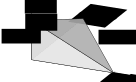
\includegraphics[width=0.65\textwidth]{./svg/integral-tetraeder}
    \caption{Gebietsintegrals für das Volumen einer schiefen Pyramide}
    \label{fig:AreaIntegTetraeder}
\end{figure}

\subsection{Gebietsintegral in Polarkoordinaten}

Abschließend wollen wir die gleiche Betrachtung noch einmal durchführen, aber mit dem Unterschied, dass die zu integrierende Fläche diesmal ein Kreis ist und wir sie nicht in kleine Rechtecke, sondern in kleine Kreissegmente zerlegen. Dies ist einfacher, als die Fläche in Rechtecke zu zerlegen. Bei der Zerlegung in Rechtecke würden im im Integral Wurzeln erscheinen, die sich meist nur schwer integrieren lassen.


In Abbildung \ref{fig:AreaIntegPolar} ist dieser Fall dargestellt. Wir gehen davon aus, dass der Kreis seinen Mittelpunkt im Koordinatenursprung besitzt und den Radius $R$ aufweist. Unsere Funktion hängt nun nicht mehr von $x$ und $y$ ab, sondern vom Abstand zum Ursprung $r$ und von Winkel mit der Abszisse $alpha$.

Das Vorgehen ist analog zum Vorgehen für Rechtecke. Wir zerlegen den Kreis mit $r\in[0,R]$ und $\alpha\in[0,,2\pi]$ in $n\cdot m$ kleine Kreissegmente mit Radius $[r_i, r_{i+1}]$ einem Winkel $[\alpha_j, \alpha_{j+1}]$. Jedes kleine Kreissegment kann näherungsweise als Rechteck aufgefasst werden mit den Seitenlängen $\Delta a = \Delta r_n$ und $\Delta b = r \Delta \alpha_n$ (siehe Skizze). Der Flächeninhalt des Kreissemgents ist daher etwa $A_{nm} = r \Delta r \Delta \alpha$. Die Stützpunkte lauten $r_i = 0 + i \Delta r_n$ und $y_j = j \Delta \alpha_m$. Wir multiplizieren den Flächeninhalt des Kreissegment mit dem Funktionswert und bilden die Summe. Es ergibt sich:

\begin{center}
    \begin{alignat*}{1}
      & \lim\limits_{(n,m) \to (\infty, \infty)} \sum\limits_{j=1}^m \sum\limits_{i=1}^n f(r_i,\alpha_j) r \Delta r_n \Delta \alpha_m  \\
    = & \int\limits_0^d \int\limits_0^\alpha f(r, \alpha) \diff{r} \diff{\alpha}
    \end{alignat*}
\end{center}

Analog kann man das Gebietsintegral auch für andere Flächen und Koordinatensystem angeben. Aus diesem Ergebnis können wir noch eine wichtige Erkenntnis ziehen. Während bei kartesischen Koordinaten nur über $x$ und $y$ integriert wurden, müssen wir in Polarkoordinaten noch einen zusätzlichen Faktor $r$ in das Integral einfügen. Je nach Koordinatensystem ist dies ein anderer Faktor, und nur im Spezialfall der kartesischen Koordinaten ist der Faktor $1$.

Wir können nun auch wieder statt festen Grenzen für $r$ diese von $\alpha$ abhängig machen. Der Vollständigkeit halber sei noch das Gebietsintegral in Polarkoordinaten analog zu den kartesischen Koordinaten definiert.

\begin{definition}{Gebietsintegral in Polarkoordinaten}{AreaIntPolar}
    Seien $u,v$ zwei einstellige Funktionen und $\alpha_1,\alpha_2\in\R$ zwei feste Zahlen. Dann wird durch $A = \left\lbrace (r,\alpha) \in \R^2 | \alpha \in [\alpha_1,\alpha_2] \land r \in [l(\alpha), u(\alpha)] \right\rbrace$ eine zweidimensionale Fläche beschrieben. Das Gebietsintegral einer Funktion $f$ über diese Fläche $A$ berechnet sich dann als:
    $$
    \int\limits_{A} f(r,\alpha) \diff{A} = \int\limits_{\alpha_1}^{\alpha_2} \int\limits_{l(\alpha)}^{u(\alpha)} f(r,\alpha) \cdot r \diff{r} \diff{\alpha}
    $$
\end{definition}

\begin{figure}
    \centering
    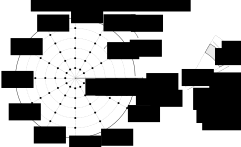
\includegraphics[width=0.95\textwidth]{./svg/integral-2d-polar}
    \caption[Gebietsintegral in Polarkoordinaten]{Graphische Interpretation eines Gebietsintegrals in Polarkoordinaten. Der Funktionswert an jedem kleinen schwarzen Punkt wird mit dem Flächeninhalt des Kreissegments multipliziert.}
    \label{fig:AreaIntegPolar}
\end{figure}

\begin{example}{Flächeninhalt des Kreises}{AreaIntPolarCircArea}
    Mithilfe des Gebietsintegral können wir auch den Flächeninhalt eines Kreises mit Radius $R$ berechnen, indem wir $f(r,\alpha) = 1$ setzen und über die Kreisfläche $r=0\dots R$ und $\alpha = 0\dots 2\pi$ integrieren:
    \begin{alignat*}{1}
        \int\limits_{A} f(x,y) \diff{A} &= \int\limits_0^{2\pi} \int\limits_0^R 1 r \diff{r} \diff{\alpha}  \\
                                        &= \int\limits_0^{2\pi} \frac{R^2}{2} \diff{\alpha} \\
                                        &= 2\pi \cdot \frac{R^2}{2} \\
                                        &= \pi R^2
    \end{alignat*}
    Damit haben wir nachgewiesen, dass der Flächeninhalt des Kreises sich tatsächlich zu $A =\pi R^2$ berechnet.
\end{example}

\section{Rechenregeln zum Differenzieren}

Um nun auch praktisch Ableitungen berechnen zu können, benötigen wir Zweierlei. Zum Einen müssen wir wissen, wie die Ableitung von Grundfunktionen (Potenz, Expoentialfunktion, Logarithmen, $\dots$) lautet. Diese kennt man entweder auswendig oder schlägt diese in Tafelwerken nach. Zum Zweiten benötigen wir noch Rechenregeln, mit denen wir aus Grundfunktionen zusammengesetzte Funktionen ableiten können. Diese sind in diesem Abschnitt kurz für einstellige Funktionen zusammengefasst.

\begin{statement}{Linearität des Differenzialoperators}{DiffOpLin}
    Der Differenzialoperator $\dd{}{x}$ ist \textbf{linear}. Sind $f$, $g$ zwei differenzierbare Funktionen und $\alpha,\beta\in\R$ zwei Konstanten, dann gilt:
    $$
        (\alpha f + \beta g)' = \alpha f' + \beta g'
    $$
\end{statement}

\begin{example}{Ableiten einer Linearkombination von Funktionen}{DiffLinCombFun}
    Die Ableitung des Polynoms $f(x) = 3x^2+6x$ ergibt sich, indem man die Monome $x^2$ und $x$ ableitet und entsprechend wieder zusammensetzt: $f'(x) = 3 * \dd{}{x} (x^2) + 6 \dd{}{x} x = 6x +6$.
\end{example}

Um ein Produkt oder Quotienten zweier Funktionen $h(x) = f(x) \cdot g(x)$ abzuleiten, betrachten wir den Grenzwert des Differenzenquotienten für $h$:

\begin{alignat*}{1}
    \dd{h}{x} &= \lim\limits_{\varepsilon\to 0} \frac{h(x+\varepsilon)-h(x)}{\varepsilon} \\
              &= \lim\limits_{\varepsilon \to 0} \frac{f(x+\varepsilon)g(x+\varepsilon)-f(x)g(x)}{\varepsilon} \\
               &= \lim\limits_{\varepsilon \to 0} \frac{f(x+\varepsilon)g(x+\varepsilon) \overbrace{-f(x)g(x+\varepsilon) + f(x)g(x+\varepsilon)}^{=0} - f(x)g(x)}{\varepsilon} \\
               &= \lim\limits_{\varepsilon \to 0} \frac{[f(x+\varepsilon)-f(x)]\cdot g(x+\varepsilon) + f(x) \cdot [g(x+\varepsilon) - g(x)]}{\varepsilon} \\
               &= \underbrace{\lim\limits_{\varepsilon \to 0} \frac{f(x+\varepsilon)-f(x)}{\varepsilon}}_{=f'(x)} \underbrace{\lim\limits_{\varepsilon\to 0} g(x+\varepsilon)}_{=g(x)\text{, da g stetig}} + f(x) \underbrace{\lim\limits_{\varepsilon \to 0} \frac{g(x+\varepsilon)-g(x)}{\varepsilon}}_{=g'(x)} \\
               &= f'(x)g(x) + f(x) g'(x)
\end{alignat*}

Damit haben wir die sogenannte Produktregel erhalten:

\begin{statement}{Produktregel}{ProdRule}
    Sind $f$ und $g$ zwei differenzierbare Funktionen, dann berechnet sich die Ableitung des Produkts der beiden Funktionen mittels der \textbf{Produktregel}:
    $$
        (f \cdot g)' = f' \cdot g + f \cdot g'
    $$
\end{statement}

\begin{example}{Ableiten eines Produkts zweier Funktionen}{CompDiffProdFun}
    Die Ableitung der Funktion $f(x) = x^2 \sin(x)$ berechnet sich mittels der Produktregel zu $f'(x) = \dd{}{x} (x^2) \cdot  \sin(x) + x^2 \dd{}{x} \sin(x) = 2x\sin(x) + x^2\cos(x)$.
\end{example}

Um eine Komposition (Verknüpfung) zweier Funktionen abzuleiten, hilft die Kettenregel, welche wir hier ohne Herleitung angeben:

\begin{statement}{Kettenregel}{ChainRule}
    Sind $f$ und $g$ zwei differenzierbare Funktionen, dann berechnet sich die Ableitung der Komposition der beiden Funktionen mittels der \textbf{Kettenregel}:
    $$
        (f \circ g)' = f' \cdot g'
    $$
    Dabei heißt $f'$ äußere Ableitung und $g'$ innere Ableitung.
\end{statement}

\begin{example}{Ableiten einer verknüpften Funktion}{CompDiffChainFun}
    \begin{itemize}
        \item Um $h(x) = (3x^2+5)^4$ abzuleiten, setzen wir $f(g) = g^4$ und $g(x) = 3x^2+5$. Deren Ableitungen sind $f'(g) = 4g^3$ (äußere Ableitung) und $g'(x) = 6x$ (innere Ableitung). Wir erhalten: $h'(x) = 4g^3 \cdot 6x = 24x(3x^2+5)^3$
        \item Die Ableitung der Funktion $h(x) = \sin(x^2)$ berechnet sich mit der äußeren Ableitung $\cos(g)$ und der inneren Ableitung $2x$ zu $h'(x) = 2x\cos(x^2)$.
    \end{itemize}
\end{example}

\begin{example}{Ableiten des Hyperbelsinus und Hyperbelkosinus}{CompDerSinh}
    Der Hyperbelsinus ist definiert als $\frac{1}{2} (e^x - e^{-x})$, der Hyperbelkosinus als $\frac{1}{2} (e^x + e^{-x})$. Mithilfe der Kettenregel finden wir $\dd{}{x}e^{-x} = -e^{-x}$ und erhalten damit für die Ableitung des Hyperbelsinus:
    $$
        \dd{}{x} \text{sinh}(x) = \frac{1}{2} (e^x-(-e^{-x})) = \text{cosh(x)}
    $$
    Analog erhält man für den Hyperbelkosinus:
    $$
        \dd{}{x} \text{cosh}(x) = \frac{1}{2} (e^x+(-e^{-x})) = \text{sinh(x)}
    $$
    Im Gegensatz zu den trigonometrische Funktionen, wo bei der Ableitung des Kosinus auf das Minuszeichen zu achten ist ($\sin(x)' = \cos(x)$, $\cos(x)' = -\sin(x)$), sind die hyperbolischen Funktionen in dieser Hinsicht symmetrisch: $\text{sinh}(x)' = \text{cosh}(x)$, $\text{cosh}(x)' = \text{sinh}(x)$.
\end{example}

\begin{example}{Ableiten eines Quotienten zweier Funktionen}{CompDiffQuotFun}
    Sei $h(x) = f(x) / g(x)$ ein Quotient zweier Funktionen. Um diesen Abzuleiten, schreiben wir $h$ als Produkt $f(x) \cdot \frac{1}{g(x)}$ und wenden die Produktregel in Kombination mit der Kettenregel an:
    \begin{alignat*}{1}
        h' &= f' \cdot \frac{1}{g} + f \cdot \left(-\frac{1}{g^2} \cdot g'\right) \\
           &= \frac{f'g - fg'}{g^2}
    \end{alignat*}
    Dies wird gelegentlich auch als \emph{Quotientenregel} bezeichnet.
\end{example}

\begin{example}{Ableitung des Tangens}{CompDiffTan}
    Die Ableitung des Tangens $\tan(x) = \frac{\sin(x)}{cos(x)}$ berechnet sich mithilfe der Quotientenregel zu:
    \begin{alignat*}{1}
        \dd{}{x} \tan(x) &= \frac{\cos(x)\cos(x)-(-\sin(x)\sin(x))}{\cos^2(x)} \\
                         &= \frac{\sin^2(x) + \cos^2(x)}{\cos^2(x)} \\
                         &= \frac{1}{\cos^2(x)} \\
                         &= 1+\frac{\sin^2(x)}{\cos^2(x)} = 1 + \tan^2(x)
    \end{alignat*}
\end{example}

Wenn eine Funktion $f(x)$ eine Umkehrfunktion $g(y) = f^{-1}(y)$ besitzt, können wir mithilfe der Kettenregel eine Formel für die Ableitung der Umkehrfunkion herleiten. Es gilt $g(f(x)) = x$, da $g$ die Umkehrfunktion zu $f$ ist. Es folgt:

\begin{alignat*}{1}
    g(f(x)) &= x \\
    \dd{}{x} g(f(x)) &= \dd{}{x} x \\
    g'(f(x)) \cdot f'(x) &= 1 \\
    g'(y) \cdot f'(x) &= 1
\end{alignat*}

Dies ist im folgenden Satz zusammengefasst:

\begin{statement}{Ableitung der Umkehrfunktion}{InverseFunDiffRule}
    Sei $f$ eine differenzierbare Funktion mit der Umkehrfunktion $f^{-1}$. Zwischen der Ableitung von $f$ und ihrer Umkehrfunktion gilt dann folgende Beziehung:
    $$
        f' \cdot (f^{-1})' = 1
    $$
\end{statement}

\begin{example}{Ableitung des Arkustangens}{CompDiffArctan}
    Die Ableitung der Arkustangensfunktion können wir mithilfe der Regel zur Ableitung von Umkehrfunktionen berechnen. Wir setzen $y = f(x) = \tan(x)$. Dann gilt:
    \begin{alignat*}{1}
        \dd{}{y} \arctan(y) &= \frac{1}{\dd{}{x} \tan(x)} \\
                            &= \frac{1}{\underbrace{1+\tan^2(x)}_{=y^2}} \\
                            &= \frac{1}{1+y^2}
    \end{alignat*}
\end{example}

\begin{example}{Ableitung des Arkussinus}{CompDiffArcsin}
    Die Ableitung der Arkussinusfunktion können wir ebenfalls mit der Regel zur Ableitung von Umkehrfunktionen berechnen. Wir erhalten:
    \begin{alignat*}{1}
        & \dd{}{x} \sin(x) \dd{}{y} \text{asin}(y) = 1 \\
        & \dd{}{y} \text{asin}(y) = \frac{1}{\cos(x)} = \frac{1}{\cos(\text{asin}(y))}
    \end{alignat*}
    Diesen Ausdruck können wir noch vereinfachen. Nach dem Satz des Pythagoras gilt $\sin^2(x) + \cos^2(x) = 1$ und damit können wir umformen:
    \begin{alignat*}{1}
        \cos(\text{asin}(x)) &= \sqrt{1 -  \sin^2(\text{asin}(x))} \\
                             & = \sqrt{1 - x^2}
    \end{alignat*}
    Also gilt für die Ableitung des Arkussinus:
    $$
        \dd{}{x} \text{asin}(x) = \frac{1}{\sqrt{1-x^2}}
    $$
\end{example}

\begin{example}{Ableitung des Arkuskosinus}{CompDiffArccos}
    Für die Ableitung der Arkuskosinusfunktion erhalten wir analog $\dd{}{y} \text{acos}(y) = -\frac{1}{\sin(\text{acos}(x))}$. Mittels $\sin(\text{acos}(x)) = \sqrt{1 - \cos^2(\text{acos}(x))}$ wird daraus:
    $$
        \dd{}{x} \text{acos}(x) = -\frac{1}{\sqrt{1-x^2}}
    $$
\end{example}


\section{Rechenregeln zum Integrieren}

Um nun auch praktisch Stammfunktionen berechnen zu können, benötigen wir Zweierlei. Zum Einen müssen wir wissen, wie die Stammfunktion von Grundfunktionen lautet. Diese kennt man entweder auswendig oder schlägt diese in Tafelwerken nach. Auf eine Stammfunktion sei aber noch einmal explizit hingewiesen, da es bei dieser oft ein Teil vergessen wird:

\begin{statement}{Stammfunktion der Hyperbel}{AntiDerHyp}
    Die Menge aller Stammfunktionen von $f(x) = \frac{1}{x}$ ist gegeben durch $F(x) = \ln(|x|) + C$
\end{statement}

Nicht vergessen werden darf der Betrag im Logarithmus -- denn $1/x$ ist sowohl für positive als auch für negative Werte definiert, $\ln(x)$ aber nur für positive Werte. Eine Weitere Stammfunktion, die manchmal hilfreich ist, lautet:

\begin{statement}{Stammfunktion der Betragsfunktion}{AntiDerSignum}
    Die Menge aller Stammfunktionen der Betragsfunktion $f(x) = \text{sgn}(x)$ ist gegeben durch $F(x) = |x| = \sqrt{x^2} + C$
\end{statement}

Zum Zweiten benötigen wir noch Rechenregeln, mit denen wir auch Stammfunktionen für aus Grundfunktionen zusammengesetzte Funktionen bilden können. Diese sind in diesem Abschnitt kurz für einstellige Funktionen zusammengefasst.

\textbf{Bei der Bildung des unbestimmten Integrals ist unbedingt auf die Integrationskonstante zu achten.} Später im Kapitel zu Differentialgleichungen werden wir feststellen, dass diese Integrationskonstante wichtig ist, da sonst viele Lösungen einer Differentialgleichung "übersehen" werden.

\begin{statement}{Linearität des Integraloperators}{IntOpLin}
    Der Integraloperator $\int \diff{x}$ ist \textbf{linear}. Sind $f$, $g$ zwei integrierbare Funktionen und $\alpha,\beta\in\R$ zwei Konstanten, dann gilt:
    $$
    \int (\alpha f + \beta g) \diff{x} = \alpha \int f \diff{x} + \beta \int g \diff{x}
    $$
\end{statement}

\begin{example}{Stammfunktion einer Linearkombination von Funktionen}{LinComAntiDer}
    Das unbestimmte Integral des Polynoms $f(x) = 3x^2+6x$ ergibt sich, indem man die Monome $x^2$ und $x$ integriert und entsprechend wieder zusammensetzt: $\int f(x) \diff{x} = 3 \int x^2 \diff{x} + 6 \int x \diff{x} = x^3 + 3 x^2 + C$.
\end{example}

Um ein Produkt zweier Funktionen zu integrieren, formen wir die Produktregel geschickt um. Wir betrachten zwei Funktion $f$ und $g$, wobei $F$ eine Stammfunktion von $f$ bezeichnet. Nach der Produktregel gilt dann:

\begin{alignat*}{1}
    (Fg)' &= F'g + Fg' \\
          &= fg + Fg'
\end{alignat*}

Beiden Seiten der Gleichung können wir nach $x$ integrieren und erhalten:

$$
  Fg = \int fg \diff{x} + \int Fg' \diff{x}
$$

Bringt man jetzt noch den rechten Summanden auf die linke Seite, erhält man die sogenannte Regel für die \emph{partielle Integration}:

\begin{definition}{Partielle Integration}{IntByParts}
    Seien $f,g$ zwei integrierbare Funktionen und $F$ eine Stammfunktion von $f$. Dann gilt für das unbestimmte Integral des Produkts beider Funktionen:
    $$
      \int f(x) \cdot g(x) \diff{x} = F(x) \cdot g(x) - \int F(x) g'(x) \diff{x}
    $$
\end{definition}

Im Gegensatz zur Produktregel gibt es einen bedeutsamen Unterschied. Die Produktregel reduziert das Problem, ein Produkt zweier Funktionen abzuleiten darauf, die beiden Einzelfunktionen abzuleiten. Das gleiche gilt für andere Ableitungsregeln. Durch sukzessive Anwendung der Ableitungsregeln kann daher die Ableitung einer zusammengesetzten Funktion immer auf die Ableitung der Grundfunktionen reduziert werden. Dies ist bei der partiellen Integration nicht der Fall. Um die Regeln erfolgreich anwenden zu können, müssen wir das Integral auf der rechten Seite bestimmen können. Im Integranden steht nun aber das Produkt der Stammfunktion und der Ableitung der anderen Funktionen. Im Allgemeinen gibt es keine Garantie dafür, dass dieses Integral einfacher zu bestimmen ist als das ursprüngliche Integral. Tatsächlich ist es so, dass selbst einfache Kombinationen von Grundfunktionen nicht mehr elementar integrierbar sind. Beispielsweise ist es nicht möglich, $\int \frac{\sin(x)}{x} \diff{x}$ nur mittels Grundfunktionen zu schreiben.

Bei der Anwendung der Produktregel sollte man daher vorher immer nachdenken, ob das auf der rechten Seite entstehende Integral lösbar sein wird. Da es sich um Produkt zweier Funktionen handelt, hat man zudem zwei Möglichkeiten für die Wahl, welche Funktion man ableitet und von welcher man die Stammfunktion bildet. Oft führt nur eine Wahl zum Ziel.

\begin{example}{Stammfunktion eines Produkts}{CompAntiDerProd}
    Gesucht ist das unbestimmte Integral von $f(x) = x e^x$. Dies wollen wir mittels partieller Integration finden. Die Funktion ist ein Produkt aus $x$ und $e^x$. Zuerst müssen wir überlegen, von welchem Faktor wir die Ableitung und von welchem Faktor wir die Stammfunktion bilden wollen. Wenn wir von $x$ eine Stammfunktion nehmen würden und von $e^x$ die Ableitung, müssten wir dann auf der rechten Seite ein Integral der Form $x^2 e^x$ lösen -- dies wird nicht einfacher sein. Wählen wir stattdessen $x$ zum Ableiten aus, wird die rechte Seite einfacher werden, da die Ableitung dann $1$ ist. Wir erhalten:
    $$
        \int x e^x \diff{x} = x e^x - \int 1 \cdot e^x \diff{x} = xe^x-e^x + C = (x-1) e^x + C
    $$
\end{example}

\begin{example}{Stammfunktion des Logarithmus}{CompAntiDerLog}
    Mittels partieller Integration kann auch der Logarithmus $f(x) = \ln(x)$ integriert werden. Dazu schreiben wir $f(x) = 1 \cdot \ln(x)$ und erhalten:
    $$
        \int 1\cdot\ln(x) = x\ln(x) - \int x/x \diff{x} = x\ln(x)-x+C = x (\ln(x) - 1) + C
    $$
\end{example}

\begin{example}{Stammfunktion des Produkts von Sinus und Kosinus}{CompAntiDerSinCos}
    Manchmal muss man nach Anwendung der partiellen Integration noch geschickt umstellen, um zum Ziel zu kommen. Für $f(x) \sin x\cos x$ erhält man beispielsweise:
    $$
        \int \sin x \cos x \diff{x} = \sin^2 x - \int \sin x \cos x \diff{x}
    $$
    Auf beiden Seiten der Gleichung kommt nun das zu bestimmende unbestimmte Integral vor. Wir können die Gleichung danach umstellen und erhalten:
    $$
        \int \sin x \cos x \diff{x} = \frac{1}{2} \sin^2 x + C
    $$
\end{example}

Analog zur Kettenregel zum Ableiten gibt es auch eine Entsprechung für das unbestimmte Integral. Um diese herzuleiten, betrachten wir zwei Funktion $f$ und $u$ und bezeichnen mit $F$ eine Stammfunktion von $f$. Für die Komposition $F \circ u$ beider Funktionen gilt nun einerseits:

$$
    (F\circ u)' = F' \cdot u' = f \cdot u'
$$

Wobei $(\dots)'$ die Ableitung nach $x$ bezeichnet. Es folgt

\begin{equation}
    \int (F \circ u)' \diff{x} = \int f \cdot u' \diff{x} \label{eq:IntPartsProof1}
\end{equation}

Andererseits gilt aber auch:

\begin{equation}
    \int (F \circ u)' \diff{x} = F \circ u = F(u) = \int f(u) \diff{u} \label{eq:IntPartsProof2}
\end{equation}

Durch Gleichsetzen von \ref{eq:IntPartsProof1} und \ref{eq:IntPartsProof1} erhalten wir die sogenannte Integration durch Substitution:

\begin{statement}{Integration durch Substitution}{IntSubst}
    Sei $f$ eine integrierbare Funktion und $u$ eine sogenannte Substitutionsfunktion. Dann gilt:
    $$
        \int f(u) \diff{u} = \int f(u(t)) u'(t) \diff{t}
    $$
\end{statement}

Bei Anwendung der obigen Regel müssen wir beachten, dass wir bei einem der beiden unbestimmten Integrale die Integrationskonstante nicht vergessen. Für die tatsächliche Berechnung ist meist das folgende Vorgehen praktikabler. Dazu müssen wir uns noch einmal daran erinnern, dass die Ableitung über den Anstieg einer Tangente definiert war. Die Tangente ist eine Gerade und der Anstieg von Gerade ist gegeben als der Quotient $\frac{\Delta y}{\Delta x}$ der Änderung des Funktionswerts und der Änderung des Arguments. Die symbolische Schreibweise $\dd{y}{x}$ können wir auch auffassen als Quotient zweier \emph{infinitesimalen} Größen $\diff{y}$ und $\diff{x}$. Diese Schreibweise nennt man \textbf{Leibniz-Notation}. Wenn wir $\dd{y}{x}$ als Bruch betrachten und damit rechnen, als wäre es ein Bruch, sind einige Formeln manchmal einfacher verständlich. Die Regel zur Ableitung der Umkehrfunktion (siehe \ref{stmt:InverseFunDiffRule}) lautet in dieser Schreibweise etwa $\dd{y}{x} \dd{x}{y} = 1$, was nach den Regeln der Bruchrechnung offensichtlich korrekt ist. Wir erhalten dann das folgende alternative Verfahren für die Integration durch Substitution:

\begin{enumerate}
    \item Wähle aufgrund der Form der zu integrierenden Funktion $f$ eine Substitution $u(x)$.
    \item Berechne die Ableitung $u'(x) = \dd{u}{x}$
    \item Forme um nach $\diff{}{x} = \frac{\diff{u}}{u'}$
    \item Ersetze nun in $\int f(x) \diff{x}$ das Argument durch $u$ und $\diff{x}$ durch $\frac{\diff{u}}{u'}$
    \item Berechne das entstehende Integral nach $u$ und ersetze abschließend wieder $u$ durch $x$.
\end{enumerate}

\begin{example}{Anwendung der Integration durch Substitution}{CompAntiDerSubst}
    Gesucht ist das Integral $\int x \cos(x^2) \diff{x}$. Dies können wir so nicht berechnen, da wir nicht wissen, wie wir einen Kosinus mit $x^2$ im Argument integrieren sollen. Es wäre schon, wenn im Argument nur $x$ stehen würde. Um das zu erreichen, wählen wir für die Substitution $u = x^2$. Die Ableitung lautet $\dd{u}{x} = 2x$. Das stellen wir um zu $\diff{x} = \frac{\diff{u}}{2x}$. Nun können wir im ursprünglichen Integral substituieren:
    \begin{alignat*}{1}
        \int x \cos(x^2) \diff{x} &= \int x \cos(u) \frac{\diff{u}}{2x} \\
                                  &= \frac{1}{2} \int \cos(u) \diff{u} \\
                                  &= \frac{1}{2} \sin(u) + C \\
                                  &= \frac{1}{2} \sin(x^2) + C
    \end{alignat*}
\end{example}

Wie bereits im vorigen Kapitel erwähnt, können gebrochenrationale Funktionen mittels Polynomdivision und Partialbruchzerlegung integriert werden. Die Polynomdivision formt eine unecht gebrochenrationale Funktion um in die Summe aus einem Polynom (was einfach zu integrieren ist) und einer echt gebrochenrationalen Funktion. Letztere kann mittels Partialbruchzerlegung in eine Summe aus Partialbrüchen zerlegt werden, die einfacher integrierbar sind. Beispielsweise haben wir im letzten Kapitel gesehen, dass sich $\frac{x}{x^2-1}$ zerlegen lässt in die beiden Partialbrüche $\frac{1/2}{x-1} + \frac{1/2}{x+1}$. Diese sind unmittelbar integrierbar: $\frac{1}{2}\ln(|x-1|) + \frac{1}{2} \ln(|x+1|) + C$.

\section{Extremwertbestimmung}

Ein Anwendungsfall der Differentialrechnung ist das Bestimmen von lokalen Extremwerten. Ein lokaler Extremwert ist gerade dadurch charakterisiert, dass die Funktion sich dort kaum ändert, also deren Ableitung verschwindet. Bevor wir den entsprechenden Satz kennenlernen, sei noch betont, dass es bei der praktischen Berechnung von Extremwerten vorkommen kann, dass ein Wert am Rand des Definitionsbereich größer oder kleiner ist als alle Funktionswert im Inneren des Definitionsbereich. Daher müssen die Randpunkte immer gesondert untersucht werden.

\begin{statement}{Notwendige Bedingung für lokalen Extremwert}{NeccCondLocEx}
    Sei $f: \R^n \to \R$ eine differenzierbare $n$-stellige Funktion. Notwendige Bedingung für das Vorliegen eines lokalen Extremwert (Minima oder Maxima) bei $\vec r_0 \in R^n$ ist es, dass dort alle partiellen Ableitungen verschwinden.
    $$
        \vec\nabla f(\vec r_0) = \vec 0
    $$
\end{statement}

Allerdings ist dies noch keine hinreichende Bedingung. Es ist möglich, eine hinreichende Bedingung für allgemeine mehrstellige Funktionen anzugeben. Da diese aber Konzepte benötigt, die bisher noch nicht behandelt wurden (es muss die Definitheit des Hessematrix untersucht werden), sei hier nur die hinreichende Bedingung für ein- und zweistellige Funktionen angegeben.

Für einstellige Funktionen muss man die zweite Ableitung untersuchen. Ist diese positiv, liegt ein Minimum vor, ist sie negativ, ein Maxima. Wenn sie gleich $0$ ist, kann man die folgende Verallgemeinerung nutzen:

\begin{statement}{Kritische Stellen einer einstelligen Funktion}{CondExSingleVar}
    Sei $n>1$ eine natürliche Zahl. An der Stelle $x_0$ liegt eine kritische Stelle der einstelligen Funktion $f$ vor, wenn gilt:
    $$
        f^{(1)}(x_0) = f^{(2)}(x_0) = \dots = f^{(n-1)}(x_0) = 0, f^{(n)}(x_0) \ne 0
    $$
    Zudem handelt es sich bei der kritischen Stelle um
    \begin{itemize}
        \item ein lokales Minimum, wenn $n$ gerade ist und $f^{(n)}(x_0) > 0$ gilt.
        \item ein lokales Maximum, wenn $n$ gerade ist und $f^{(n)}(x_0) < 0$ gilt.
        \item eine Sattelstelle, wenn $n$ ungerade ist.
    \end{itemize}
\end{statement}

\begin{example}{Berechnung lokaler Extremstellen}{LocExUnivarFun}
    \begin{itemize}
        \item Gesucht sind die lokalen Extremstellen von $f(x) = x \ln x$. Die Ableitung lautet $f'(x) = \ln x + 1$. Setzt man diese $0$, erhält man als Kandidaten für die Extremstelle $x_0 = 1/e$. Um herauszufinden, ob es sich um ein Minimum oder Maximum handelt, bilden wir die zunächst die zweite Ableitung: $f''(x) = 1 / x$. Wir setzen den Extremstellenkandidaten ein und erhalten $f''(1/e) = e$. Dies ist offensichtlich eine positive Zahl, folglich handelt es sich an der Stelle $1/e$ um ein lokales Minimum.
        \item Die Funktion $f(x) = -x^4$ hat offensichtlich ein lokales Maximum bei $x_0 = 0$. Die erste Ableitung $f'(x) = -4x^3$ verschwindet bei $0$. Doch auch die zweite Ableitung $f''(x) = -12x^2$ ist identisch $0$. Um zu bestätigen, dass es sich tatsächlich um ein Maximum handelt, leiten wir weiter ab. Die dritte Ableitung $f'''(x) = -24x$ verschwindet ebenfalls, die  vierte Ableitung $f''''(x) = -24$ nicht. In diesem Fall ist $n=4$ eine gerade Zahl, es handelt sich also tatsächlich um eine Extremstelle. Da $f''''(0) = -24 < 0$ handelt es sich zudem um ein Maximum.
    \end{itemize}
\end{example}

Für zweistellige Funktionen muss man die zweiten partiellen Ableitungen an der Kandidatenstelle für den Extremwert bilden und wie folgt prüfen:

\begin{statement}{Lokaler Extremwert einer mehrstelligen Funktion}{CondExBiVar}
    Sei $f: \R^2 \to \R$ eine zweistellige Funktion und $(x_0,y_0)\in R^2$ eine Kandidatenstelle für den Extremwert, also $f_x(x_0,y_0) = f_y(x_0,y_0) 0$. Dann liegt bei $(x_0,y_0)$ eine Extremstelle vor, falls gilt:
    $$
        \Delta = f_{xx} f_{yy} - f_{xy}^2 > 0
    $$
    Die partiellen Ableitungen sind dabei an der Kandidatenstelle auszuwerten. Ferner gilt,
    \begin{itemize}
        \item $(x_0,y_0)$ ist ein Minimum, wenn $f_{xx}(x_0,y_0) > 0$ gilt.
        \item $(x_0,y_0)$ ist ein Maximum, wenn $f_{xx}(x_0,y_0) < 0$ gilt.
    \end{itemize}
    Ist $\Delta < 0$, so liegt eine Sattelstelle vor. Für $\Delta = 0$ ist keine Aussage möglich.
\end{statement}

\begin{example}{Extremwert einer zweistelligen Funktion}{CompBivarEx}
    Gesucht sind die Extremstellen von $f(x,y) = xy + \frac{1}{x} + \frac{1}{y}$. Wir berechnen zuerst die partiellen Ableitungen: $f_x = y-\frac{1}{x^2}$, $f_y = x-\frac{1}{y^2}$, $f_{xx} = \frac{2}{x^3}$, $f_{yy} = \frac{2}{y^3}$, $f_{xy} = 1$. Als Kandidaten für Extremstellen kommen Stellen in Betracht, wo beide ersten partiellen Ableitung verschwinden. Aus $f_x = f_y = 0$ folgt $y=\frac{1}{x^2}$ sowie $x=\frac{1}{y^2}$. Setzen wir die erste Gleichung in die zweite ein, erhalten wir $y=\frac{1}{\left(1/y^2\right)^2} = y^4$ und daraus $y=1$. Damit ist $x=1/1^2 = 1$. Die einzige Kandidatenstelle ist $(x,y) =(1,1)$. Um herauszufinden, ob dort tatsächlich eine Extremstelle vorliegt, berechnen wir die Größe $\Delta = f_{xx}(1,1)f_{yy}(1,1) - f_{xy}(1,1)^2 = 2\cdot2 - 1^2 = 3$. Da $\Delta \ne 0$, liegt eine Extremstelle vor. Da zudem $f_{xx}(1,1) = 2 > 0$ gilt, handelt es sich um ein lokales Minimum. In Abbildung \ref{fig:ExCompBivarEx} sieht man die Extremstelle auch deutlich in der Konturliniendarstellung.
\end{example}

\begin{figure}
    \centering
    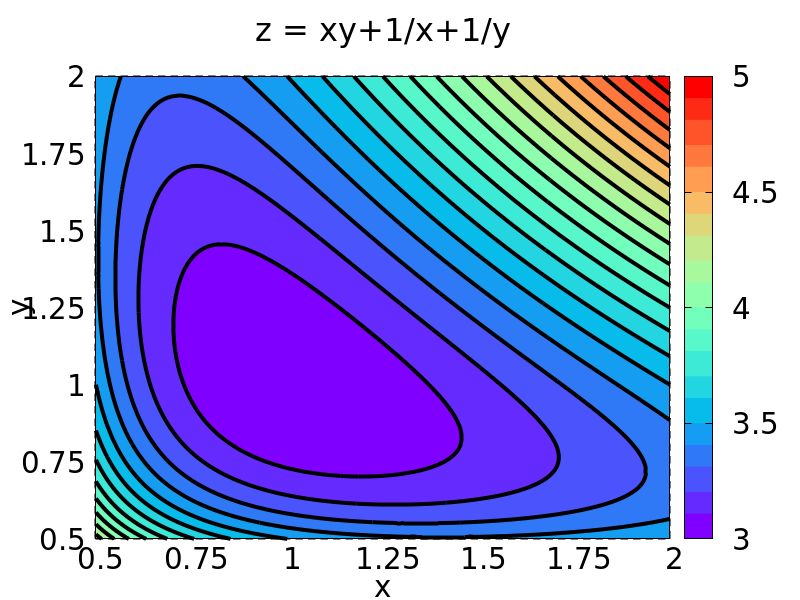
\includegraphics[width=0.65\textwidth]{./gnuplot/contour-field-extrem-values}
    \caption[Extremwertbestimmung mittels Konturlinien]{Konturlinien der zweistelligen Funktion aus Beispiel \ref{ex:CompBivarEx}. Man erkennt die Extremstelle deutlich an der geschlossenen Konturlinie.}
    \label{fig:ExCompBivarEx}
\end{figure}
